\chapter{Числовой пример решения задачи алгоримом на основе метода ветвей и границ}\label{app:bnb_algorithm}

Рассмотрим пример решения задачи в комбинаторной задачи. Пусть задан отрезок $\alpha$ длиной $L = 50$ с концами в точках $a_0$ и $a4$ с координатами $l_0 = 0$ $l_4 = 50$. Внутри данного отрезка имеется множество точек размещения $A = \{a_i\}, i = 1, 2, 3$ с координатами $l_1 = 20, l_2 = 30, l_3 = 40$. 

Задано множество БС $S = \{ s_j \} , j = 1, 2$. Каждой станции приписаны параметры $s_j = \{ r_j, \{R_{jq}\}\}$.  Для $s_1$ задано $r_1 = 25$, $R_{10} = 62, R_{12} = 35, R_{14} = 31$. Для $s_2$ задано $r_2 = 9$, $R_{20} = 31, R_{12} = 28, R_{24} = 39$.
На концах отрезка размещены шлюзы $s_0$ и $s_4$. Радиус связи шлюзов для соединения с БС $R_{01} = R_{41} = 62$ и $R_{02} = R_{42} = 39$. 


Необходимо разместить БС $s_1$ и $s_2$, т.е. найти такую расcтановку $P^*$, которая минимизирует функционал недопокрытия $f(P)$ \cref{eq:part3_objective_function}

\textbf{Решение полным перебором.}

Общее количество размещения двух станций по трем точкам равна $\gamma = C^2_3 \cdot 2! = 6$.

Процесс решения задачи представлен в виде бинарного дерева поиска. Каждый узел пронумерован согласно правилам \textit{\textbf{процедуры 1}}. Оранжевым цветом указаны листья, в которых либо получили расстановку станций, либо на данном множестве $G_\nu$ набор фиксированных и запрещенных переменных $\pi_{ij}$ делает недопустимым любое размещение (обозначено символом $\varnothing$).


\begin{table}[h!]\centering
  \begin{tabular}{|c|c|c|}\hline
      
      Расстановка, $P$ & Недопокрытие, $f(P)$ & Номер узла дерева\\
      \hline
      $P_1$ & 11 & 3\\
      \textit{\textbf{$P_2$}} & \textit{\textbf{1}} & \textit{\textbf{5}}\\
      $P_3$ & 11 & 9\\
      $P_4$ & 11 & 11\\
      $P_5$ & 6 & 15\\
      $P_6$ & 21 & 19\\
      \hline

\end{tabular}\caption{Решение полным перебором}\label{app:brute_force_solution}
\end{table}

В таблице \cref{app:brute_force_solution} представлены полученные в ходе решения расстановки. Все расстановки пронумерованы в соответсвии с порядком их нахождения. Оптимальным решением $P^*$ с минимальным значением функции \cref{eq:part3_P} является допустимая расстановка $P_2$.


\textbf{Решение с помощью МВиГ.}

Теперь решим пример данной задачи в соответствии с разработанным МВиГ. Так как мы не учитываем ограничения на стоимость и величину задержку, допустимая расстановка должна удовлетворять только требованиям 1 и 2, а также условию размещения всех имеющихся БС.


За начальный рекорд примем длину всего отрезка $\widehat{P} = L = 50$.

Исследование множества $G_0$.  



\fixme{ПЕРЕДЕЛАТЬ РИСУНОК МЕТОД ВЕТВЕЙ И ГРАНИЦ}


\chapter{Числовой пример оптимального размещения базовых станций сети с линейной топологией в виде экстремальной задачи в комбинаторной форме}\label{app:bnb_solution}



Дано:
\begin{itemize}
  \item линейный участок $L =300$ метров;
  \item множество точек размещения $|A| =8$;
  \item множество БС $|S| =8$;
  \item протокол IEEE 802.11n;
  \item ограничение на суммарную стоимость $T =0.001$с;
  \item интенсивность входящих пакетов $\lambda = 1000$ 1/c;
  \item средний размер входящих пакетов $w = 1500$ байт;
  \item отклонение от оптимального решения, $\varepsilon=0.5$%
\end{itemize}

Рассмотрим пример задачи размещения базовых станций вдоль линейного участка для организации БШС. В данном приложении будет представлен пример решения задачи для БШС на базе протокола IEEE 802.11n. 





Задан линейный участок $L =300$ метров. На данном участке в ходе обследования местности были выбраны восемь возможных точек размещения базовых станций, $|A| =8$. Координаты $l_i$ точек размещения представлены в таблице \cref{tab:placement_point}.

\begin{table}[h!]\centering
  \begin{tabular}{|c||c|c|c|c|c|c|c|c|}\hline
      
      Точки размещения, $a_i$ &	$a_1$&	$a_2$&	$a_3$&	$a_4$&	$a_5$&	$a_6$&	$a_7$& $a_8$ \\
      \hline
      Координаты, $l_i$ &	43&	72&	98&	150&	178&	201&	269&	280\\
      \hline

\end{tabular}\caption{Координаты точек размещения}\label{tab:placement_point}
\end{table}

На рынке представлен широкий спетр технических устройств от компаний Cisco, Mikrotik и т.д. позволяющий организовывать сеть в открытой местности и учитывающий климатические сложности на нефтегазовых месторождениях, такие как предельные температуры, сила ветра и т.д. Под БС в нашей задаче будем понимать точку доступа с антеннами для покрытия заданной области и антеннами для обеспечения связи с соседними станциями БШС. 

В ходе этапа выбора комплекса технических средств были выбраны восемь БС. Множество станций $|S| = 8$. Каждой БС преписаны паспортные характеристики антенн, пропускная способность точки доступа и итоговая стоимость станции. Стоимость взята условная, чтобы не указывать реальные цены производителя на время написания диссертации и курс валют. Будем рассматривать БШС для задачи мониторинга, то есть с каналом передачи на верхний уровень, UpLink. Рабочая частота 2,4 ГГц. Для каждой БС будем использовать пропускную способность для модуляции и схемы кодирования MCS7.  В таблице \cref{tab:sta_parameters} представлены параметры БС.

\begin{table}[h!]\centering
  \begin{tabular}{|c||c|c|c|c|c|c|c|c|}\hline
      
      S&	$P_{tr}^R$&	$G_{tr}^R$&	$P_{recv}^R$&	$L$&	$P_{recv}^r$&	$G_{recv}^r$&	$p$&	$c$ \\
      \hline
      №&	дБм&	дБ&	дБм&	дБ&	дБм&	дБ&	Мбит/с&	у.е. \\
      \hline
      1&	20&	4&	-77&	1&	-77&	3&	72,2& 24 \\
      2&	19&	4&	-77&	1&	-73&	4&	72,2&	20 \\
      3&	19&	4&	-77&	1&	-77&	5&	72,2&	24 \\
      4&	18&	4&	-77&	1&	-77&	3&	72,2&	24 \\
      5&	19&	4&	-77&	1&	-77&	4&	72,2&	28 \\
      6&	19&	4&	-77&	1&	-74&	4&	72,2&	24 \\
      7&	20&	4&	-77&	1&	-73&	4&	72,2&	20 \\
      8&	19&	4&	-77&	1&	-77&	4&	72,2&	20 \\
      \hline

\end{tabular}\caption{Параметры базовых станций. $P_{tr}^{R}$ -- мощность направленной антенны, $G_{tr}^R$ -- усиление направленной антенны, $P_{recv}^R$ -- чувствительность направленной антенны, $L$  -- потери в антенном кабеле и разъемах, передающего тракта, $P_{recv}^r$ -- чувствительность всенаправленной антенны, $G_{recv}^r$ -- усиление всенаправленной антенны,  $p$ – пропускная способность, $c$ – стоимость}\label{tab:sta_parameters}
\end{table}

На концах участка размещены шлюзы $s_0 $ и $s_{m+1}$ с параметрами (таблица \cref{tab:app_gateway_parameters}):

\begin{table}[h!]\centering
  \begin{tabular}{|c||c|c|c|c|}\hline
      
      Шлюз&	$P_{tr}^R$&	$G_{tr}^R$&	$P_{recv}^R$&	$L$ \\
      \hline
      №&	дБ&	дБ&	дБ&	дБ \\
      \hline
      $s_0 $&	20&	5&	-77&	1 \\
      $s_{m+1}$&	20&	5&	-77&	1 \\
      \hline

\end{tabular}\caption{Параметры шлюзов}\label{tab:app_gateway_parameters}
\end{table}

Для расчета области покрытия необходимо задаться характеристиками устройств, с которых будет собираться информация (таблица \cref{tab:app_user_device_parameters}).


\begin{table}[h!]\centering
  \begin{tabular}{|c||c|c|c|}\hline
      
    Устройство&	$P_{tr}^ud$&	$G_{tr}^ud$&	$L$ \\
    \hline
    &	дБ&	дБ&	дБ	 \\
    \hline
    &	9&	1&	0 \\

    \hline

\end{tabular}\caption{Параметры устройств}\label{tab:app_user_device_parameters}
\end{table}


Итоговое размещение БС должно удовлетворять заданным ограничениям:
\begin{itemize}
  \item на стоимость $C = 76$;
  \item на межконцевую задержку сети $T =0.001$ с.
\end{itemize}
Для расчета времени межкоцневой задержки, будем считать, что на каждую БС поступает трафик с интенсивностью $\lambda = 1000$ 1/с. Средний размер поступающих пакетов $w=1500$ байт.

Для поиска последовательности топологий задано отклонение $\varepsilon=0.5$\% от найденного оптимального значения.

\subsection{Расчет радиуса связи и радиуса покрытия станций}

По формуле (5) рассчитаем радиус покрытия для каждой станции (таблица \cref{tab:app_sta_coverage}) и радиусы связи между станциями и со шлюзами (таблица \cref{tab:app_sta_link} и таблица \cref{tab:app_gateway_link}).

\begin{table}[h!]\centering
  \begin{tabular}{|c||c c c c c c|}\hline
      
      Станция&	$S_1$& $S_2$& $S_3$& $S_4$& $S_5$& $S_{m+1}$\\
      \hline
      $r_j$, м&	48&	43&	38&	43&	43&	0\\
      \hline

\end{tabular}\caption{Рассчитанные радиусы покрытия}\label{tab:app_sta_coverage}
\end{table}

\begin{table}[h!]\centering
  \begin{tabular}{|c|c c c c c c c|}\hline
      
      $R_{jq}$, м&	$S_1$& $S_2$& $S_3$& $S_4$& $S_5$& $S_0$& $S_{m+1}$\\
      \hline
      $S_1$& --&	76&	96&	96&	76&	76&	76\\
      $S_2$& 85&	--&	85&	85&	68&	68&	68\\
      $S_3$& 76&	60&	--&	76&	60&	60&	60\\
      $S_4$& 85&	68&	85&	--&	68&	68&	68\\
      $S_5$& 85&	68&	85&	85&	--&	68&	68\\

      \hline
\end{tabular}\caption{Рассчитанные радиусы связи базовых станций}\label{tab:app_sta_link}
\end{table}

\begin{table}[h!]\centering
  \begin{tabular}{|c|c c c c c|}\hline
      
      $R_{jq}$, м&	$S_1$& $S_2$& $S_3$& $S_4$& $S_5$ \\
      \hline
      $S_0$& 96&	85&	76&	85&	85\\
      $S_{m+1}$& 96&	85&	76&	85&	85\\
      \hline
\end{tabular}\caption{Рассчитанные радиусы связи шлюзов}\label{tab:app_gateway_link}
\end{table}


В таблице \cref{tab:app_bnb_solution_result} представлены результаты решения размещения станций. Для заданной $\varepsilon=1\%$, т.е. $d=2$ был получены последовательности расстановок для \underline{\textit{\textbf{задач 2, 3 и 4}}} расчета оценок с помощью задачи ЦЛП, задачи «О ранце» и ЛП. В таблице представлены рекорды «недопокрытия», стоимости и задержки сети, а также размещения станций, число пройденных узлов дерева а и время счета.
Задача ЦЛП и задача о ранце решались с помощью Optimization Toolbox Matlab, а задача ЛП решалась с помощью библиотеки c исходным кодом Scipy Python. Как видно из результатов оценка, полученная с помощью задачи ЛП менее точная, приходится обходить большее количество узлов для нахождения рекордов по сравнению с методом оценки «недопокрытия» с помощью \underline{\textit{\textbf{задач 2 и 3}}}. В итоге возрастает итоговое количество пройденых узлов. В свою очередь метод ЛП имеет свое преимущество, так как время счета меньше.


\fontsize{10pt}{10pt}\selectfont
\begin{longtable}[c]{| c | c | c | c | c  c  c  c  c  c  c|}
    \caption{Сравнения оценок «недопокрытия» для задачи ЦЛП и ЛП}\label{tab:app_bnb_solution_result}\\

    \hline
    \multirow{2}{*}{№} & \multirow{2}{*}{Рекорд, м} & \multirow{2}{*}{Стоимость, у.е.} & \multirow{2}{*}{Задержка, сек} & \multicolumn{7}{|c|}{Размещение} \\\cline{5-11}

    &&&& $a_1$&	$a_2$&	$a_3$&	$a_4$&	$a_5$&	$a_6$&	$a_7$ \\
    \hline
    1&	1&	65&	0,03244&	$S_1$&	-&	$S_4$&	-&	-&	$S_5$&	- \\
    2&	1&	65&	0,03244&	$S_1$&	-&	$S_5$&	-&	-&	$S_4$&	- \\
    3&	1&	65&	0,03244&	$S_4$&	-&	$S_1$&	-&	-&	$S_5$&	- \\
    4&	0&	65&	0,03244&	$S_4$&	-&	$S_5$&	-&	-&	$S_1$&	- \\
    5&	1&	65&	0,03244&	$S_5$&	-&	$S_1$&	-&	-&	$S_4$&	- \\
    6&	0&	65&	0,03244&	$S_5$&	-&	$S_4$&	-&	-&	$S_1$&	- \\
    7&	1&	65&	0,03244&	-&	$S_1$&	$S_4$&	-&	-&	$S_5$&	- \\
    8&	1&	65&	0,03244&	-&	$S_1$&	$S_5$&	-&	-&	$S_4$&	- \\
    9&	1&	65&	0,03244&	-&	$S_1$&	-&	$S_4$&	-&	$S_5$&	- \\
    10&	0&	65&	0,03244&	-&	$S_1$&	-&	$S_4$&	-&	-&	$S_5$ \\
    11&	1&	65&	0,03244&	-&	$S_4$&	$S_1$&	-&	-&	$S_5$&	- \\
    12&	0&	65&	0,03244&	-&	$S_4$&	$S_5$&	-&	-&	$S_1$&	- \\
    13&	1&	65&	0,03244&	-&	$S_4$&	-&	$S_1$&	-&	$S_5$&	- \\
    14&	0&	65&	0,03244&	-&	$S_4$&	-&	$S_1$&	-&	-&	$S_5$ \\
    15&	1&	65&	0,03244&	-&	$S_5$&	$S_1$&	-&	-&	$S_4$&	- \\
    16&	0&	65&	0,03244&	-&	$S_5$&	$S_4$&	-&	-&	$S_1$&	- \\
    \hline \hline

    \multicolumn{2}{|c|}{\thead{Метод оценки \\ «недопокрытия» \\ справа}} & \multicolumn{3}{|c|}{ЦЛП}&	\multicolumn{3}{|c|}{Задача «О ранце»}&	\multicolumn{3}{|c|}{ЛП} \\
    \hline  \hline
    \multicolumn{2}{|c|}{\thead{Число \\ пройденных \\ узлов}}& \multicolumn{3}{|c|}{934}&	\multicolumn{3}{|c|}{934}&	\multicolumn{3}{|c|}{1590} \\  
    \hline
    \multicolumn{2}{|c|}{\thead{Время \\ счета,\\ сек}}& \multicolumn{3}{|c|}{5,412}&	\multicolumn{3}{|c|}{5,136} &	\multicolumn{3}{|c|}{3,613} \\
    \hline

    \hline
\end{longtable}
\normalsize

\chapter{Численный пример оптимального размещения базовых станций для обслуживания заданного множества рассредоточенных объектов}\label{app:milp_place_solution}
Рассмотрим пример для оптимизационной задачи выбора набора размещаемых станций и определения мест их размещения.
Задано множество рассредоточенных объектов $A_1$, $|A_1| = 4$ и шлюз (таблица \cref{tab:part2_placement_coordinates}).

\begin{table}
    \centering
    \captionsetup{justification=centering} % выравнивание подписи по-центру
    \caption{Координаты размещения}\label{tab:part2_placement_coordinates}
    \begin{tabular}{|l|c|c|}
        \toprule
        0   & (7,4) & \textbf{Координаты шлюза} \\
        \midrule
        1   & (1, 5)& \textbf{Координаты объектов}  \\
        2   & (4.5, 4) & \\
        3   & (6, 3) & \\
        4   & (3.5, 5) & \\
        \midrule
        5   & (2, 4) & \textbf{Координаты размещения станций}  \\
        6   & (5, 5) & \\
        7   & (2, 6) & \\
        8   & (6, 5.5) & \\
        \bottomrule
    \end{tabular}
\end{table}

Задано множество $A_2$ возможных мест расположения станций, $|A_2| = 4$. Все вершины представлены на Рисунке \ref{fig:part2_coordinates}.
 
\begin{figure}[ht]
    \centerfloat{
        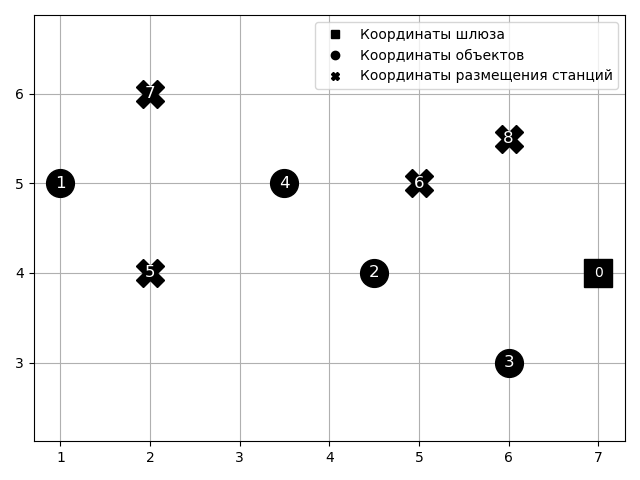
\includegraphics[scale=0.75]{part2_coordinates.png}
    }
    \caption{Координаты размещения}\label{fig:part2_coordinates}
\end{figure}

Задано ограничение по мощности для кадого объекта (таблица \ref{tab:part2_object_capacity}).

\begin{table}
    \centering
    \captionsetup{justification=centering} % выравнивание подписи по-центру
    \caption{Координаты размещения}\label{tab:part2_object_capacity}
    \begin{tabular}{|c|cccc|}
        \toprule
        Объекты   & 1 & 2 & 3 & 4 \\
        \midrule
        Мощность  & 10 & 15 & 17 & 18 \\
        \bottomrule
    \end{tabular}
\end{table}

Задано множество типов станций (таблица \ref{tab:part2_station_types_1}).

\begin{table}
    \centering
    \captionsetup{justification=centering} % выравнивание подписи по-центру
    \caption{Множество типов станций}\label{tab:part2_station_types_1}
    \begin{tabular}{|c|c|c|c|c|}
        \toprule
        Тип & Мощность, $\vartheta_j$ & Радиус покрытия, $r_j$  & Радиус связи, $R_j$ & Стоимость, $c_j$ \\
        \toprule
        1   & 80 & 1 & 6 & 70 \\
        2  & 100 & 2 & 5 & 75 \\
        3  & 100 & 2 & 5 & 75 \\
        \bottomrule
    \end{tabular}
\end{table}

Необходимо разместить станции таким образом, чтобы минимизировать их  суммарную общую стоимость.
Построим граф сети $H$ для данного набора типов станции. Матрица смежности представлена на рисунке \cref{fig:part2_adjacency_matrix}
 
\begin{figure}[ht]
    \centerfloat{
        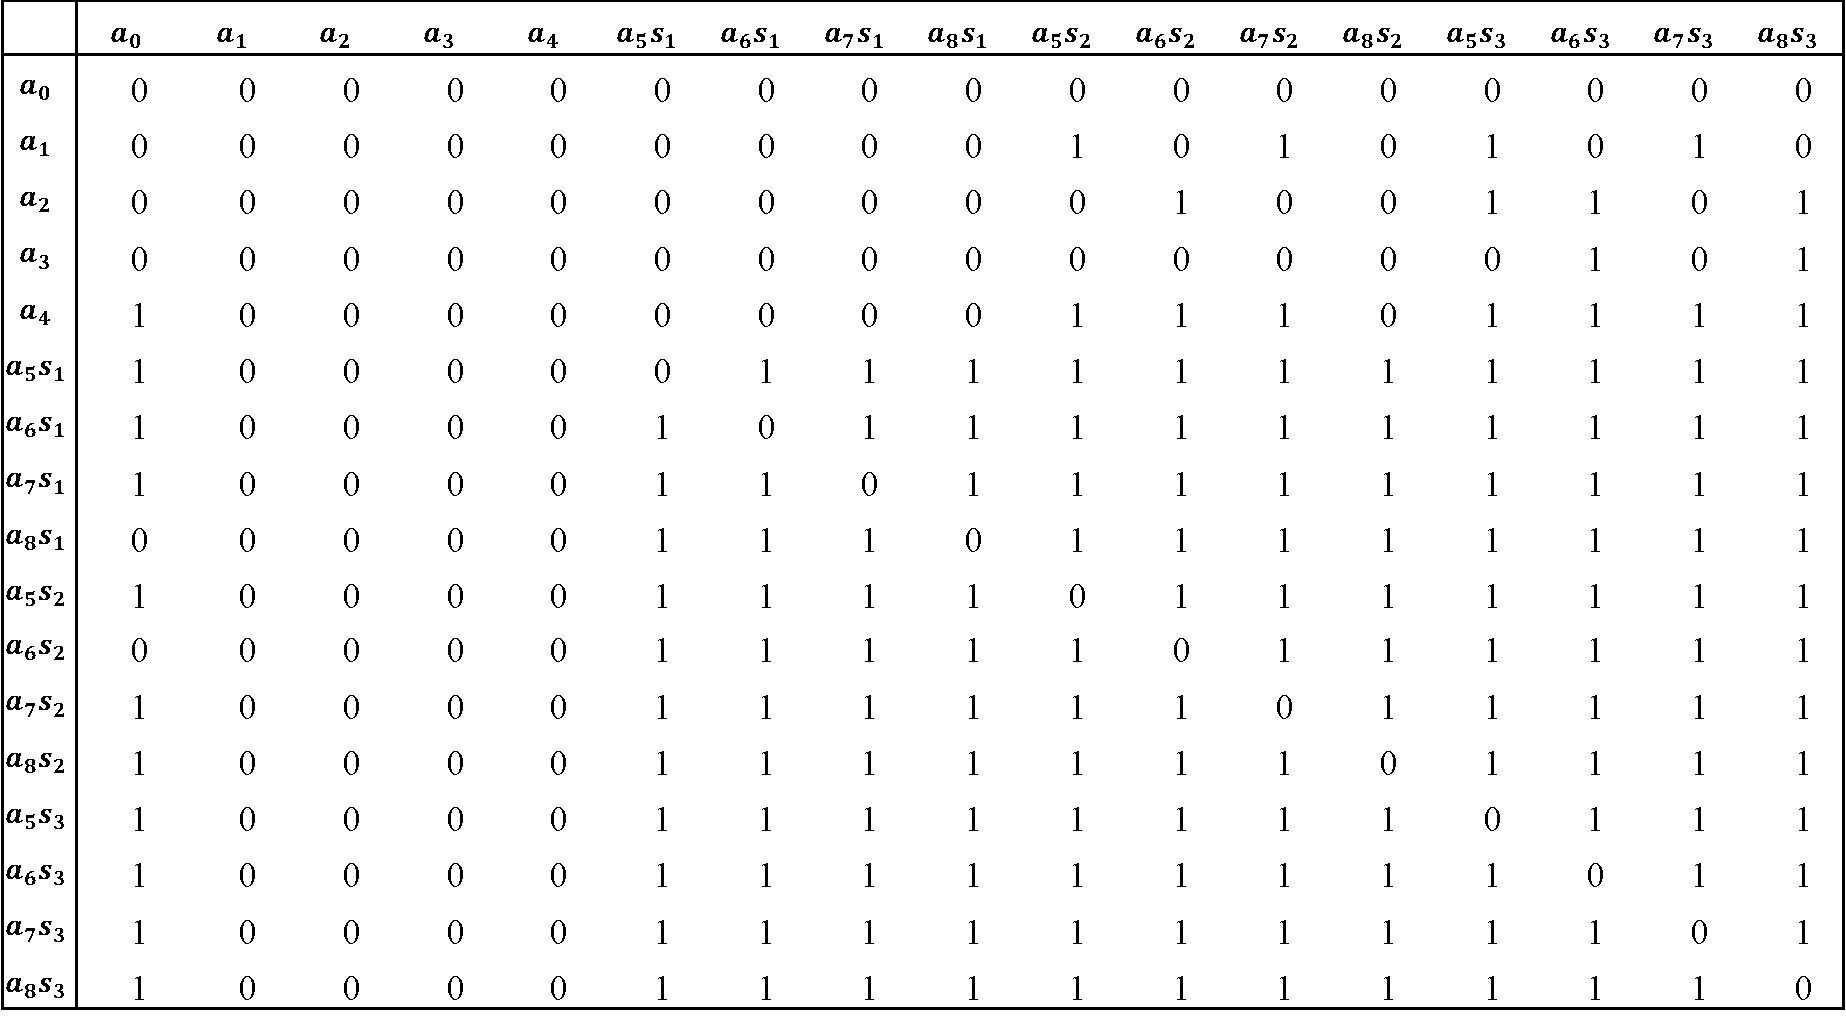
\includegraphics[scale=0.5]{part2_adjacency_matrix.pdf}
    }
    \caption{Координаты размещения}\label{fig:part2_adjacency_matrix}
\end{figure}

% \begin{table}
%     \centering
%     \captionsetup{justification=centering} % выравнивание подписи по-центру
%     \caption{Матрица смежности графа $H$}\label{tab:part2_adjacency_matrix}
%     \begin{tabular}{|c|c|c|c|c|c|c|c|c|c|c|c|c|c|c|c|c|}
%         \toprule
%         a_0 & a_1 & a_2 & a_3 & a_4 & a_5s_1 & a_6s_1 & a_7s_1 & a_8s_1 & a_5s_2 a_6s_2 & a_7s_2 & a_8s_2 & a_5s_3 & a_6s_3 & a_7s_3 & a_8s_3 \\
%         \toprule
%         1   & 80 & 1 & 6 & 70 \\
%         2  & 100 & 2 & 5 & 75 \\
%         3  & 100 & 2 & 5 & 75 \\
%         \bottomrule
%     \end{tabular}
% \end{table}


На основе матрицы смежности полученного графа запишем систему равенств и неравенств\cref{eq:part2_1.5, eq:part2_1.6, eq:part2_1.7, eq:part2_1.8, eq:part2_1.9, eq:part2_1.10} и решим задачу частично целочисленного ЛП.
В ходе решения мы получили следующее размещение станции (Рисунок \cref{fig:part2_solution})

\begin{figure}[ht]
    \centerfloat{
        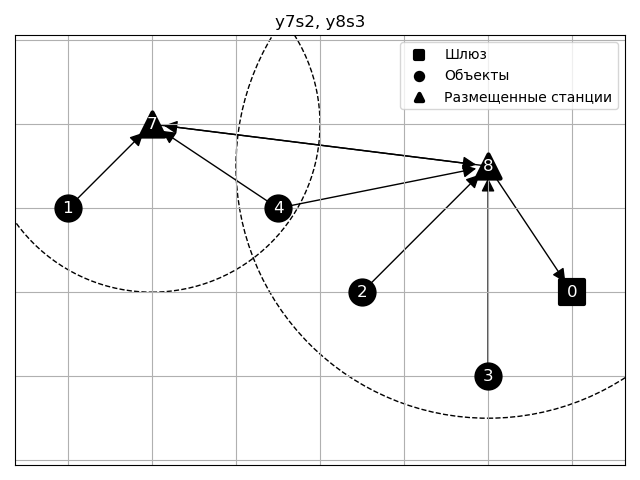
\includegraphics[scale=0.75]{part2_solution.png}
    }
    \caption{Координаты размещения}\label{fig:part2_solution}
\end{figure}

Из графика видно, что были размещены на точках 7 и 8 две станции типа 2 и 3, соответственно.
Решением задачи является суммарная стоимость равная:
$f=160$.





% \section{Результаты численного эксперимента}

Алгоритмы построения графов $H$ были запрограммированы на языке Python. Задачи, сформулированные на основании графов $H$ в виде соответствующих задач математического программирования, были решены пакетом Optimization Toolbox MATLAB.
В таблице 4 представлены результаты времени счета задач частично целочисленного ЛП для различных случаев числа мест размещения станций и числа объектов. Для каждого случая было проведено по 10 примеров.

\begin{table}
    \centering
    \captionsetup{justification=centering} % выравнивание подписи по-центру
    \caption{Множество типов станций}\label{tab:part2_station_types}
    \begin{tabular}{|c|c|c|}
        \toprule
        Количество & Количество мест  & Среднее время 
        \tabularnewline объектов, $n_1$ & размещения станций, $n-n_1$ &  счета, сек.  \\
        \toprule
        4   & 3 & 12,34 \\
        4   & 4 & 12,42 \\
        4   & 5 & 12,31 \\
        6   & 6 & 11,20 \\
        8   & 7 & 11,27 \\
        10  & 7 & 12,32 \\
        12  & 10 & 12,51 \\
        14  & 7 & 12,42 \\
        17  & 8 & 12,18 \\
        21  & 8 & 12,53 \\
        25  & 8 & 14,22 \\
        \bottomrule
    \end{tabular}
\end{table}


\chapter{Численный пример оптимального размещения базовых станций сети с линейной топологией в виде задачи ЦЛП}\label{app:ilp_solution}
В этой секции представлен численный пример решения данной задачи.
% This section shows one simple case of the problem.

Задан линейный участок $L$ с длиной 300 с количеством $n=7$ точек размещения. Координаты точек размещения представлены в таблице \cref{tab:part3_placed_point}.  Задан бюджет размещения $C=130$. Центарльная частота $f = 2437$ МГц. 

\begin{table}[h!]\centering
  \begin{tabular}{|c||c|c|c|c|c|c|c|}\hline
    $a_i$ & $a_1$ &  $a_2$ & $a_3$ & $a_4$ & $a_5$ & $a_6$ & $a_7$ \\ \hline \hline
    Координата & 29 & 40 & 95 & 139 & 181 & 230 & 273 \\ \hline
\end{tabular}\caption{Точки размещения участка с длиной $L = 300$.}\label{tab:part3_placed_point}
\end{table}

Задано множества базовых станций $m = 8$ с параметрами представленными в таблице \cref{tab:part3_BS}. Также в таблице представлены параметры шлюзов и контролируемых объектов. Параметры объектов необходимы для расчета радиусов покрытия станций.

\begin{table}[b]\centering
  \begin{tabular}{|c||c|c|c|c|c|c|c|}\hline
    BS & $P_{tr}^R$ &  $G_{tr}^R$ & $P_{recv}^R$ & $P_{recv}^r$ & $G_{recv}^r$ & $c$ \\ \cline{2-1} \cline{3-1} \cline{4-1} \cline{5-1}  \cline{6-1} \cline{7-1}
     & дБм & дБ & Дбм & дБм & дБ & у.е.  \\ \hline
    1 & 20 & 5 & -69 & -67 & 5 & 40 \\ 

    2 & 19 & 5 & -67 & -67 & 5 & 28 \\ 

    3 & 18 & 5 & -69 & -67 & 5 & 45 \\ 

    4 & 19 & 5 & -69 & -67 & 6 & 22 \\ 

    5 & 19 & 5 & -67 & -67 & 5 & 21 \\ 

    6 & 20 & 5 & -69 & -67 & 5 & 40 \\ 

    7 & 19 & 5 & -67 & -67 & 5 & 28 \\

    8 & 18 & 5 & -69 & -67 & 5 & 45 \\ \hline \hline  

    &  $G_{recv}^R$ & $P_{recv}^R$ &  & & $P_{tr}^r$ & $G_{tr}^r$ \\  \cline{2-1} \cline{3-1} \cline{6-1} \cline{7-1} 

    Шлюз& дБ & дБм & & Объект & дБм & дБ  \\  \cline{2-1} \cline{3-1}  \cline{6-1} \cline{7-1}

    &  5 & -69 & &  & 15 & 2  \\ \hline

  \end{tabular}\caption{Параметры базовых станций, шлюзов и объектов.}\label{tab:part3_BS} 
\end{table}

\textbf{Расчет радиса связи между станциями}
Базовые станции оснащены направленной антенной с высоким коэффициентом усиления для связи с соседними станциями.
Для расчета потерь между станциями $j$ и $q$ воспользуемся формулой (\ref{eq:part3_L_fs_from_link_budget}):

\begin{displaymath}
  L_{fs}^{jq} = P_{tr}^R(j) - L_{tr} + G_{tr}^R(j) + G_{tr}^R(q) - L_{recv} - SOM - P_{recv}^R(q).
\end{displaymath}


Потери на кабелях приемникп $ L_{recv} $ и передатчике $ L_{tr} $ примем равным 1 дБ и запас на замирания сигнала $ SOM = 10 $ дБ.

Let us carry out an example of the calculation communication link between stations $ s_1 $ and $ s_2 $:
Для примера расчетаем радиус связи между станциями $ s_1 $ и $ s_2 $:

\begin{align}
  \begin{aligned}
  L_{fs}^{12} = P_{tr}^R(1) - L_{tr} + G_{tr}^R(1) + G_{tr}^R(2) - L_{recv} - SOM - P_{recv}^R(2)= \\
  = 20 - 1 + 5 + 5 - 1 - 10 - (-69) = 87 (dB).
  \end{aligned}
\end{align}

Для расчета канала связи необходимо использовать формулу \cref{eq:part3_D}. Несущая частота $ f = 2437 $ МГц и коэффициент для расчета потерь $ K = -27,55 $:

\begin{align}
  \begin{aligned}
  R_{jq} = 10^{\left(\frac{L_{fs}^{jq} - 20\lg{F} - K}{20}\right)}
  = 10^{\left(\frac{87 - 20\lg{2437} - (-27.55)}{20}\right)} = 174 (m).
  \end{aligned}
\end{align}

В таблице \cref{tab:part3_Rjq} приведены расчеты максимальных радиусов связи между всеми станциями $ s_j $, $ j = 1, ..., m $ и шлюзом $ s_ {m + 1} $.

\begin{table}[h!]\centering
  \begin{tabular}{|c||c|c|c|c|c|c|c|c|c|}\hline
      $R_{jq}$ & $s_1$ & $s_2$ & $s_3$ & $s_4$ & $s_5$ & $s_6$ & $s_7$ & $s_8$ & $s_{m+1}$ \\ \hline \hline

      $s_1$ &--& 174& 219& 219& 174& 219& 174& 219& 219\\ 
      $s_2$ &195& --& 195& 195& 155& 195& 155& 195& 195\\ 
      $s_3$ &174& 138& --& 174& 138& 174& 138& 174& 174\\ 
      $s_4$ &195& 155& 195& --& 155& 195& 155& 195& 195\\ 
      $s_5$ &195& 155& 195& 195& --& 195& 155& 195& 195\\ 
      $s_6$ &219& 174& 219& 219& 174& --& 174& 219& 219\\
      $s_7$ &195& 155& 195& 195& 155& 195& --& 195& 195\\ 
      $s_8$ &174& 138& 174& 174& 138& 174& 138& --& 174\\ 
      \hline

\end{tabular}\caption{Рассчитанные радиусы связи между станциями}\label{tab:part3_Rjq}
\end{table}

\textbf{Расчет радиуса покрытия}

% Для покрытия заданного участка базовая станция оснащена всенаправленной антенной с выходной мощностью $ P_{tr}^r $ и усилением $ G_{tr}^r$. Потери в кабеле $ L_ {tr} $ равно 1.

% To cover a given section, the base station is equipped with an isotropic antenna with output power $ P_ {tr} ^ r $ and gain $ G_ {tr} ^ r $ is equal to 0. The cable loss $ L_ {tr} $ is equal to 1.

% A coverage area depends on a base station, as well as user device characteristics. Let us consider a user device with an antenna sensitivity $P_{RX} = -67$ dBm and gain $G_{RX} = 0$. Loss $L_{RX}$ is equal to 0.
Расчет проводится аналогично расчета радиусу связи между станциями. 
Потери в свободном простанстве для канала между $j$-ой станции и контролируемым объектом

\begin{displaymath}
  L_{fs}^{j} = P_{tr}^r(j) - L_{tr}  - SOM - P_{RX}. 
\end{displaymath}


Пример расчечта радиуса покрытия для  $1$-ой станции:

\begin{align}
    \begin{aligned}
  L_{fs}^{1} = P_{tr}^r + G_{tr}^r + G_{recv}^r(1) - L_{recv}(1)  - SOM - P_{recv}^r(1) = \\
 = 15+2+5-1-(-67)-10 = 78 \text{ (дБ)}.
    \end{aligned}
\end{align}

\begin{displaymath}
  r_{1} = 10^{\left(\frac{78 - 20\lg{2437} - (-27.55)}{20}\right)} = 77 \text{ (м)}.
\end{displaymath}

Рассчитанные радиусы покрытия для всех станций $ s_j $, $ j = \overline{1, m} $ представлены в таблице \cref{tab:part3_rj}).

\begin{table}[h!]\begin{center}
  \begin{tabular}{|c||c|c|c|c|c|c|c|c|}\hline
      STA & $s_1$ & $s_2$ & $s_3$ & $s_4$ & $s_5$ & $s_6$ & $s_7$ & $s_8$\\ \hline \hline

      $r_{j}$ & 77 & 77 & 77 & 87 & 77 & 77 & 77 & 77\\ \hline

\end{tabular}\caption{Рассчитанные радиусы покрытия станций}\label{tab:part3_rj}
\end{center}\end{table}

Задача ЦЛП решена с помощью Optimization Toolbox MatLab. Таблица \cref{tab:part3_ilp_solution} содержит все полученные целочисленные решения.


\begin{table}[h!]\tiny\centering
  \begin{tabular}{|c||c|c|c|c|c|c|c||c|c|}\hline
    $a_i$ & $a_1$ &  $a_2$ & $a_3$ & $a_4$ & $a_5$ & $a_6$ & $a_7$  & Покрытие & Цена \\ \hline 
    Координаты & 29 & 40 & 95 & 139 & 181 & 230 & 273 & м & у.е.\\ \hline \hline
    Целлочисленное решение 1 & $s_1$ & $s_2$ & $s_6$ & -- & -- & -- & $s_4$ & 286 & 130\\ 
    Целлочисленное решение 2 & $s_4$ & -- & $s_5$ & $s_7$ & -- & -- & $s_2$ & 289 & 99\\
    Оптимальное решение & $s_4$ & $s_2$ & -- & -- & $s_1$ & -- & $s_5$ & 300 & 111 \\ \hline
\end{tabular}\caption{Решение задачи ЦЛП.}\label{tab:part3_ilp_solution}
\end{table}



\chapter{Сравнения оценок «недопокрытия» для задачи 2, 3 и 4}\label{app:task_234}

В таблице \cref{tab:app_estimate_comparison} приведены результаты вычислительного эксперимента, показывающего время решения \underline{\textit{\textbf{задач 2, 3, 4}}} и относительную точность \underline{\textit{\textbf{задачи 3, 4}}} по отношению к \underline{\textit{\textbf{задаче 2}}}.
Для непокрытого участка заданной длины $|\beta| = 50$, варьируя количеством неразмещенных станций, а также количеством свободных мест размещения рассчитаем оценку недопокрытия при бюджетном ограничении $C=600$.
Как видно из результатов расчетов, представляется целесообразным для решения задач большой размерности использовать в качестве оценки $w_2 (G_\nu )$ \underline{\textit{\textbf{задачу 3}}}, так как время ее расчета в виде задачи линейного программирования существенно ниже с учетом высокой точности.


\fontsize{8pt}{8pt}\selectfont
\begin{longtable}[c]{| c | c | c | c | c | c | c | c |c | c |}
    \caption{Сравнения оценок «недопокрытия» для задачи ЦЛП и ЛП}\label{tab:app_estimate_comparison}\\

    \hline
    \multirow{2}{*}{\thead{Количество \\
        точек \\
        размещения, \\ $m$}}
    & \multirow{2}{*}{\thead{Количество \\
        свободных \\
        станций, \\ $|S_\beta|$}}

    & \multicolumn{2}{|c|}{ЦЛП} 
    & \multicolumn{3}{|c|}{\thead{Задача \\
    о ранце}} 
    & \multicolumn{3}{|c|}{ЛП} \\\cline{3-10}
 
    &&\rotatebox{270}{Время расчета, сек } 
    &\rotatebox{270}{Недопокрытие, $z$}
    &\rotatebox{270}{Время расчета, сек} 
    &\rotatebox{270}{Недопокрытие, $z$}
    &\rotatebox{270}{Точность, \%}
    &\rotatebox{270}{Время расчета, сек} 
    &\rotatebox{270}{Недопокрытие, $z$}
    &\rotatebox{270}{Точность, \%}\\

    \hline
    5&	6&	0,3250&	436,00&	0,3214&	426,00&	97,71&	0,0047&	436,00&	100,00 \\
    5&	8&	0,3218&	431,00&	0,3582&	398,00&	92,34&	0,0045&	431,00&	100,00 \\
    8&	10&	0,3765&	395,00&	0.3621&	375,00&	94,94&	0,0094&	395,00&	100,00 \\
    8&	12&	0,3746&	390,00&	0.2977&	347,00&	88,97&	0,0094&	390,00&	100,00 \\
    12&	15&	0,3363&	339,00&	0.2960&	309,00&	91,15&	0,0114&	339,00&	100,00 \\
    12&	17&	0,4072&	336,00&	0.3456&	283,00&	84,23&	0,0136&	336,00&	100,00 \\
    18&	20&	0,3558&	265,00&	0.3407&	265,00&	100,00&	0,0121&	265,00&	100,00 \\
    18&	25&	0,3794&	260,00&	0.3096&	259,00&	99,62&  0,0169&	257,60&	99,08 \\
    25&	30&	0,3177&	246,00&	0.3576&	246,00&	100,00&	0,0222&	244,33&	99,32 \\
    25&	45&	0,3539&	229,00&	0.3556&	229,00&	100,00&	0,0494&	226,40&	98,86 \\
    30&	50&	0,2994&	225,00&	0.3146&	225,00&	100,00&	0,0570&	224,13&	99,61 \\
    30&	100& 0,5179& 223,00& 0,5177& 223,00& 100,00& 0,1513& 218,75& 98,09 \\
    \hline
\end{longtable}
\normalsize


